\usetheme{metropolis}

\usepackage{appendixnumberbeamer}

\usepackage{booktabs}
\usepackage[scale=2]{ccicons}

\usepackage{pgfplots}
\usepgfplotslibrary{dateplot}

\usepackage{xspace}
\newcommand{\themename}{\textbf{\textsc{metropolis}}\xspace}

\metroset{titleformat frame=smallcaps}

% Add section numbers in TOC
% https://tex.stackexchange.com/a/44998/173708
\setbeamertemplate{section in toc}[sections numbered]

%%% Local Variables:
%%% mode: latex
%%% TeX-master: t
%%% End:


% make background color for title of the slides green
\definecolor{OilGainsGreen}{RGB}{85, 130, 5}    % Fidelity green normal
\setbeamercolor{frametitle}{bg=OilGainsGreen}   % do not change foreground color

% set folder for figures
\graphicspath{{figs/}}


% remove the [rt] keyword. Offset and increase to maximum size
% https://tex.stackexchange.com/a/412707/173708
\titlegraphic{%
  \begin{picture}(0,0)
    \put(154,-114){\makebox(0,0){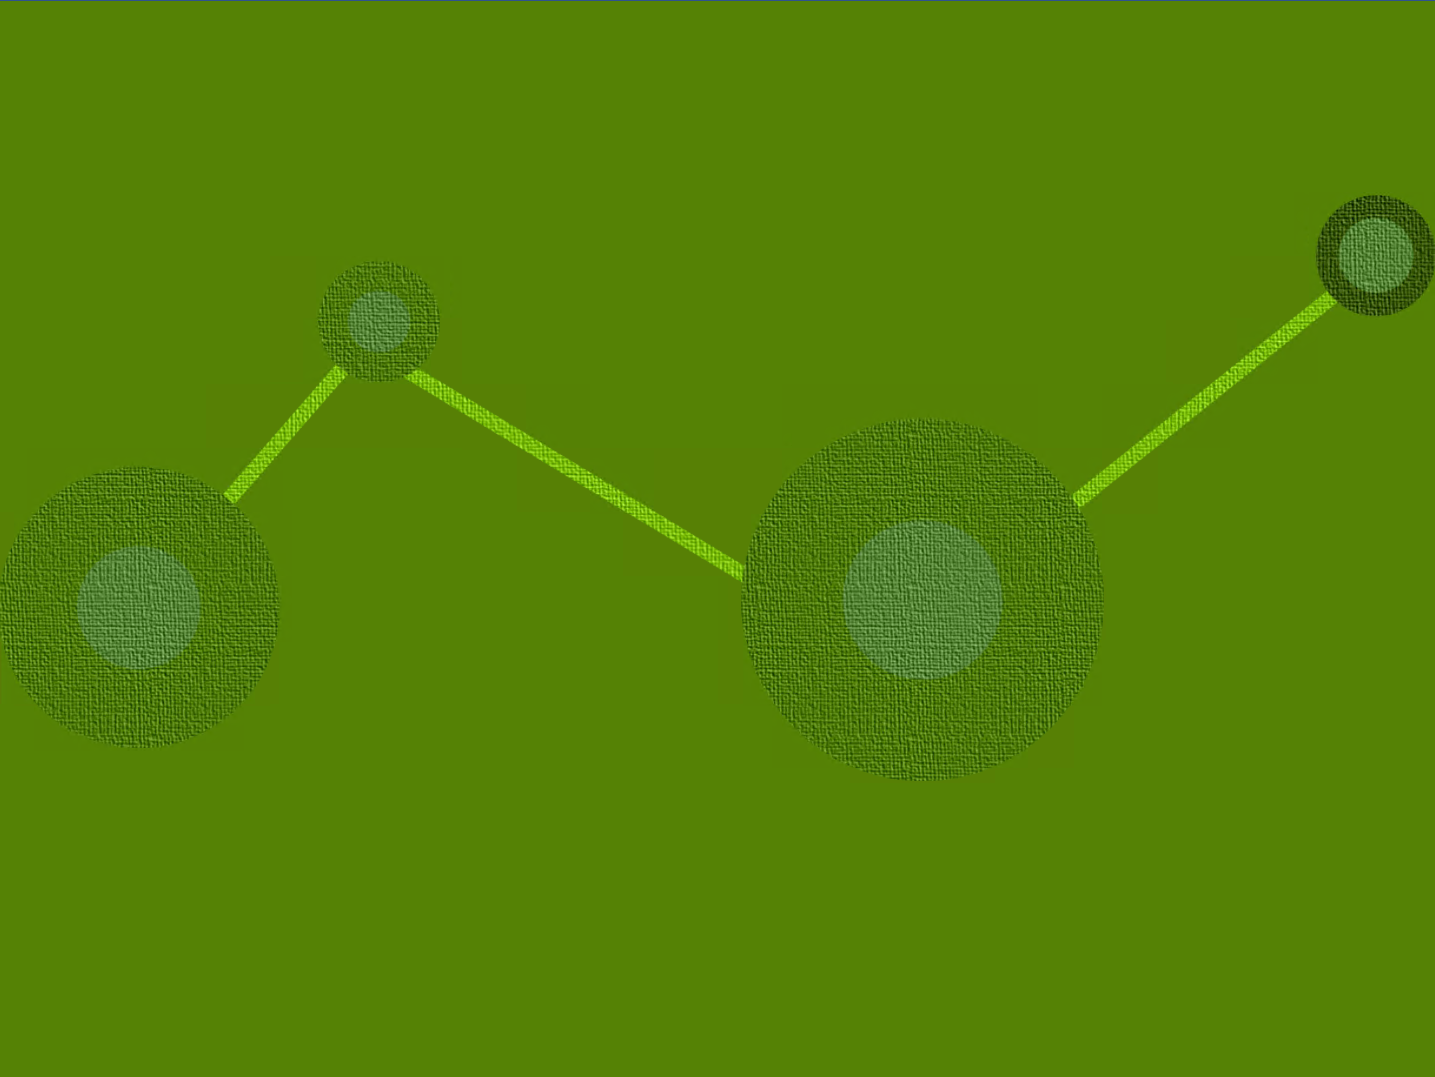
\includegraphics[width=\paperwidth,height=\paperheight]{OilGainsTitleSlide2}}}
  \end{picture}}


% change color of title and subtitle
\definecolor{OilGainsGreen}{RGB}{85, 130, 5}  % Fidelity green normal
\setbeamercolor{title}{fg=white,bg=OilGainsGreen}
\setbeamercolor{subtitle}{fg=yellow,bg=OilGainsGreen}
\setbeamercolor{author}{fg=white,bg=OilGainsGreen}
\setbeamercolor{date}{fg=white,bg=OilGainsGreen}
\setbeamercolor{institute}{fg=yellow,bg=OilGainsGreen}

% change color of the progress bar
\definecolor{blueucl}{RGB}{0,87,156} %which is the color of my university
\setbeamercolor{progress bar}{fg=blueucl}
\setbeamercolor{title separator}{fg=lightgray} % color of the title separator
\setbeamercolor{progress bar in head/foot}{fg=blueucl}
\setbeamercolor{progress bar in section page}{fg=blueucl}

